\section{Background - Its descriptive chapter;  Keep it short and precise; Make it so that reader can get the main point}
The service mesh is a fairly new architectural concept to unify multiple services and ideas under one independently managed part of the backend architecture. Many of these services and ideas are nothing new, but their combination and easy accessibility makes their usage more compelling. In a blog entry Richard A. Hogan from Nginx said "some of the loudest buzz in the IT industry during 2018 was around the concept of service mesh" \citep{nginx-service-mesh}. To understand why the service mesh is suddenly of such big interest in the industry, it is important to look at how the backend architecture evolved especially microservices. The term microservice was discussed as part of a workshop of software architects in 2011 and ratified later in 2012 as the main term describing the architectural style of breaking up the business logic into small self-contained parts \citep{fowler2014microservices}. Until then, it was common to develop a huge integrated system with many functions that could not be run independently, commonly known as monoliths \citep{dragoni2017microservices}. Big Internet companies like Google and Microsoft already separated their architecture into smaller parts for maintainability, independent deployments, speed, and horizontal scaling \citep{micro-at-google}, but it was not quite the same as microservices and many SME (Small and medium-sized enterprises) stuck to the concept of building a monolith.  In their paper "Microservices: The Journey So Far and Challenges Ahead" \cite{jamshidi2018microservices}, make a list of important technologies for the evolution of microservices. \Cref{fig:history-micro} is a representation of this, where only stable releases are taken into account (not beta or alpha versions) and the coloring is meant to highlight technologies in the same (or similar) area.
\begin{figure}[ht]
    \centering
    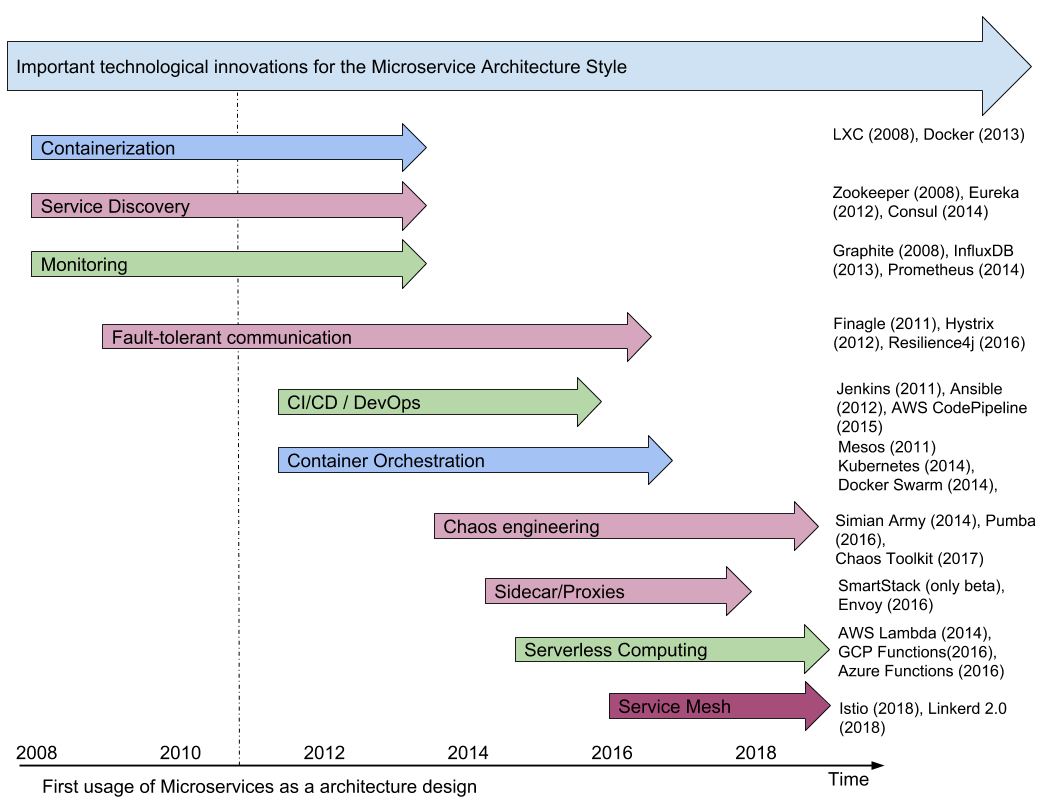
\includegraphics[width=150mm]{figures/history-diagram.png}
    \caption{\textbf{Please correct dates and insert important software !!!!!!!} History of Microservice Technologies[Inspired by: source }
    \label{fig:history-micro}
\end{figure}
Without going into too much detail, it is important to notice the common similarities of early innovations. So beginning in the 2008th there was this push for enabling microservices in their most basic form. Abstracting them from the OS level via containers, monitoring them and setting up a system, which can automatically discover the microservices. Later, beginning in 2012, CI/CD pipelines and container orchastration were seen as the next big challenge. CI is the intgration and 